\chapter{UNIFIED MODEL ASSEMBLY FRAMEWORK\label{chapter:umaf}}
The Unified Model Assembly Framework (UMAF) is a collection of algorithms designed to transform source code programs into executable models of the real-world system under study.
In order to accomplish this task, UMAF will use the original source code program as well as variable grounding information from supporting texts in order to build executable models that are linked to real-world variables.
Domain scientists commonly desire for scientific models to facilitate the inspection of the computations contained in the model and for the wiring of variables in the model to be easily observable.
To meet these desires, the form of the executable models produced by UMAF will be a function network, a graphical model that shows variables as nodes wired together by the computations of the model, while hiding the actual computations performed in function nodes that can be inspected as necessary.
UMAF will then utilize information from supporting texts to link the source code variables in the function network to real-world variables in the physical system of interest.
This process is termed \textit{grounding the variable nodes}, and once this process is complete the function network is now a Grounded Function Network (GrFN), which is the final form of models produced by UMAF.

Due to the function network structure GrFNs are executable and, since they are executable, GrFNs can also be analyzed by functional analysis methods.
As a side-effect of the variable grounding process, competing GrFNs can be structurally compared upon the wiring of their variables, allowing for comparisons to be made amongst competing GrFNs of the same real-world system.
The structure of a GrFN also allows for the wiring of variables, and computations among variables to be altered as need be by domain scientists, which also leads to the ability of GrFNs of different systems to be composed into a larger GrFN of the over-arching real-world system.
These properties combine to show that UMAF is able to convert models contained in source code programs and described in published texts into GrFNs that can be executed, analyzed, compared, altered, and composed by domain modelers who wish to have as many capabilities as possible when designing scientific models of the real-world systems they study.

\begin{figure}[!htbp]
    \label{fig:automates_pipeline}
    \centering
    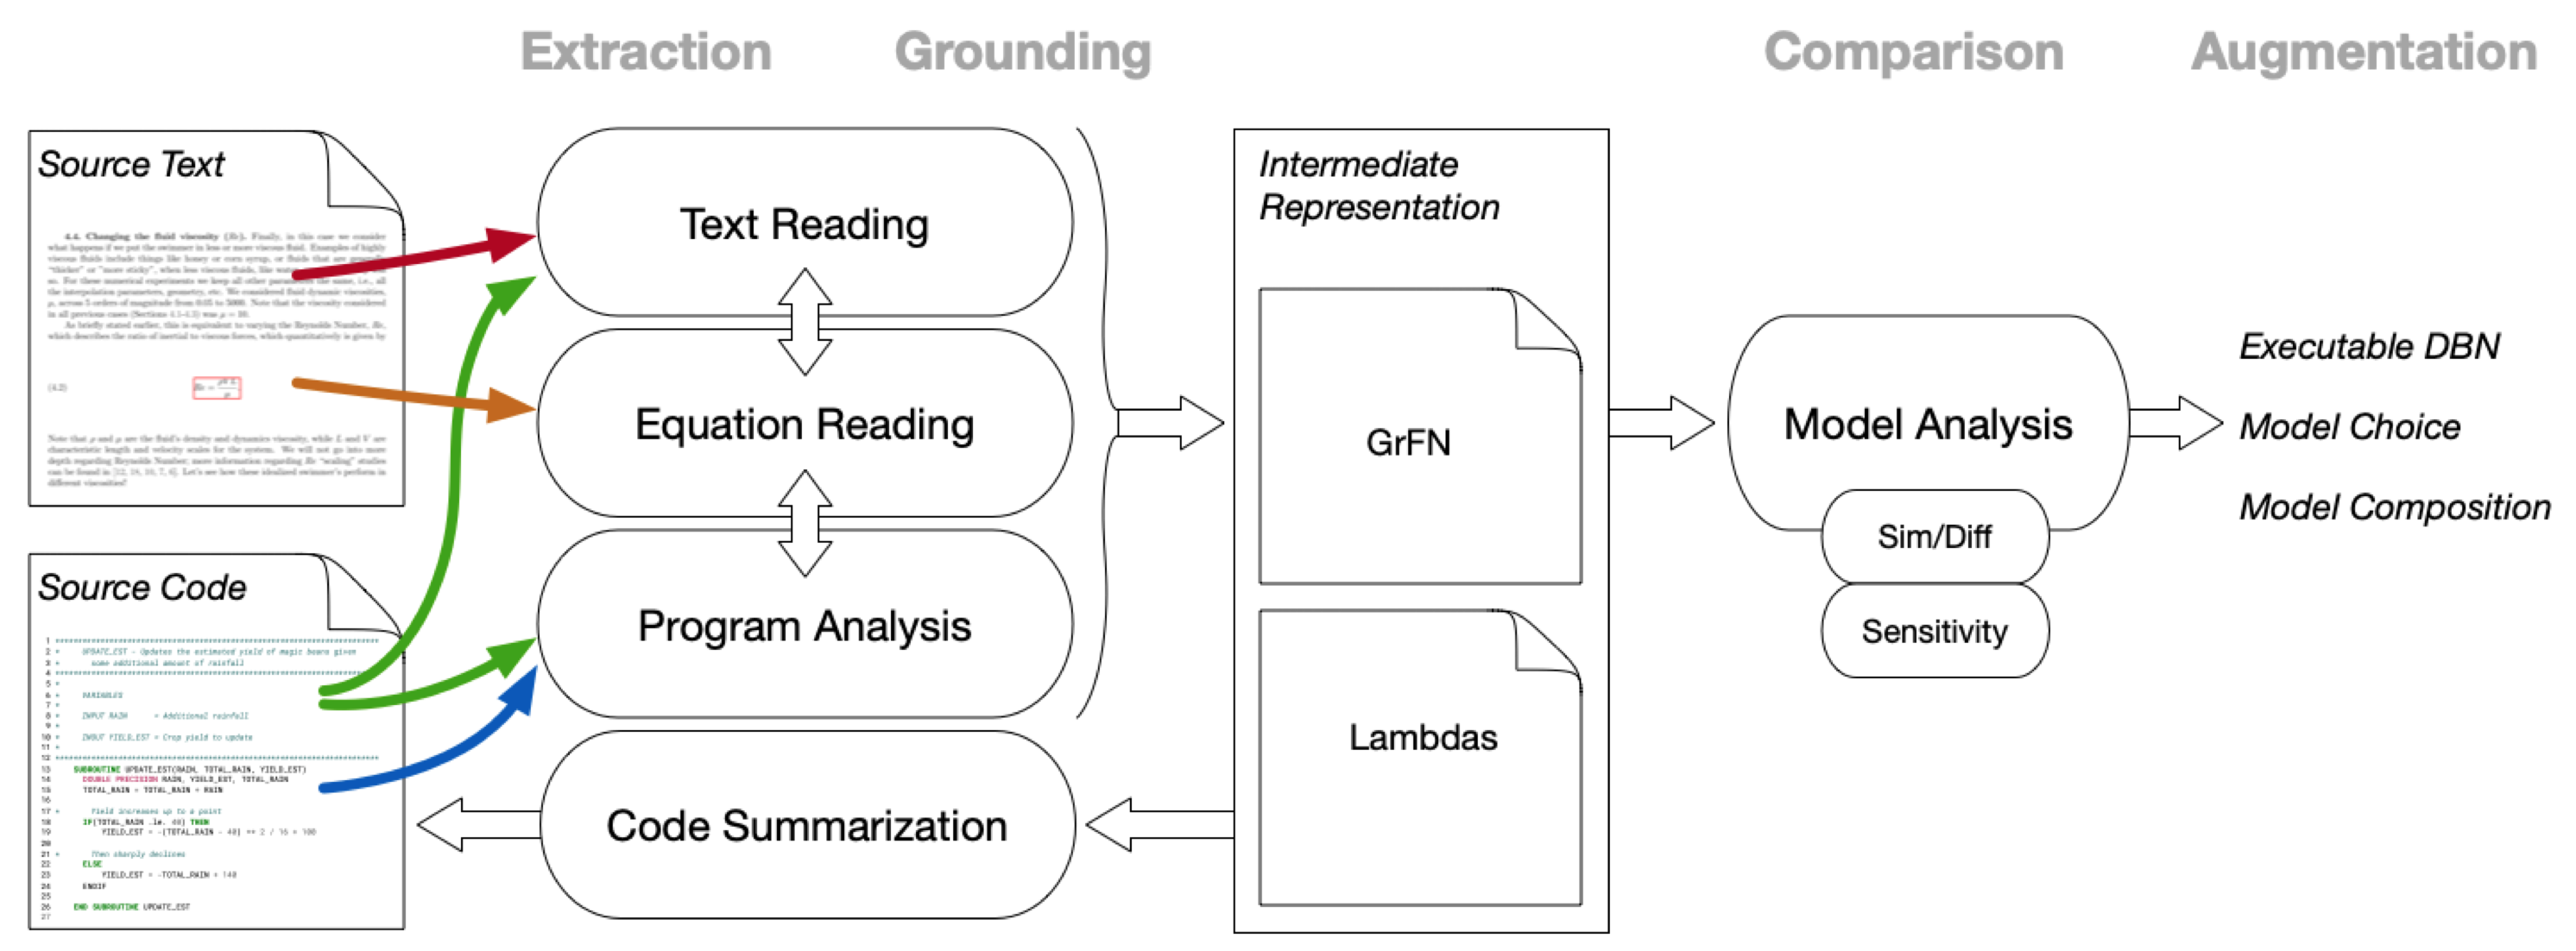
\includegraphics[width=.8\columnwidth]{automates_pipeline}%
    \caption[The AutoMATES Pipeline]{A view of the wiring of all the modules of the AutoMATES pipeline. This figure shows the various inputs of the separate \textit{Program Analysis}, \textit{Text Reading}, and \textit{Equation Reading} modules. UMAF is contained in the portions of the pipeline comprising the intermediate representation and model analysis sections. Different colored arrows on the pipeline inputs where blue represents program source code, green represents program documentation, red represents free text found in published works, and orange represents equation images found in published works. As shown in the pipeline, the outputs from the three first modules are combined into an intermediate representation that is used by UMAF to generate models that can then be used in the model analysis phase.}
\end{figure}

This chapter will begin with a background section that covers the modules of the AutoMATES pipeline (Fig~\ref{fig:automates_pipeline}) that provide input to UMAF.
Once the inputs to UMAF have been fully covered I will proceed to discuss how UMAF utilizes these inputs to perform the translation to GrFN as shown in Fig~\ref{fig:umaf_diagram}, as well as discuss how the grounding process is performed upon variables in a GrFN.
The main purpose for transforming source code programs into GrFNs is to facilitate model analysis, and many of the model analysis methods we seek to support require probabilistic models that allow for probabilistic inference and sampling techniques to be performed on the model.
Therefore the third section of this chapter will focus on connecting the semantics of UMAF's GrFN models to the world of probabilistic graphical modeling.
Finally, the chapter will conclude with an evaluation study that discusses the current program idiom coverage of UMAF as a means to evaluate what source code programs can be converted by UMAF into GrFN representations of scientific models.

\begin{figure}[!htbp]
    \label{fig:umaf_diagram}
    \centering
    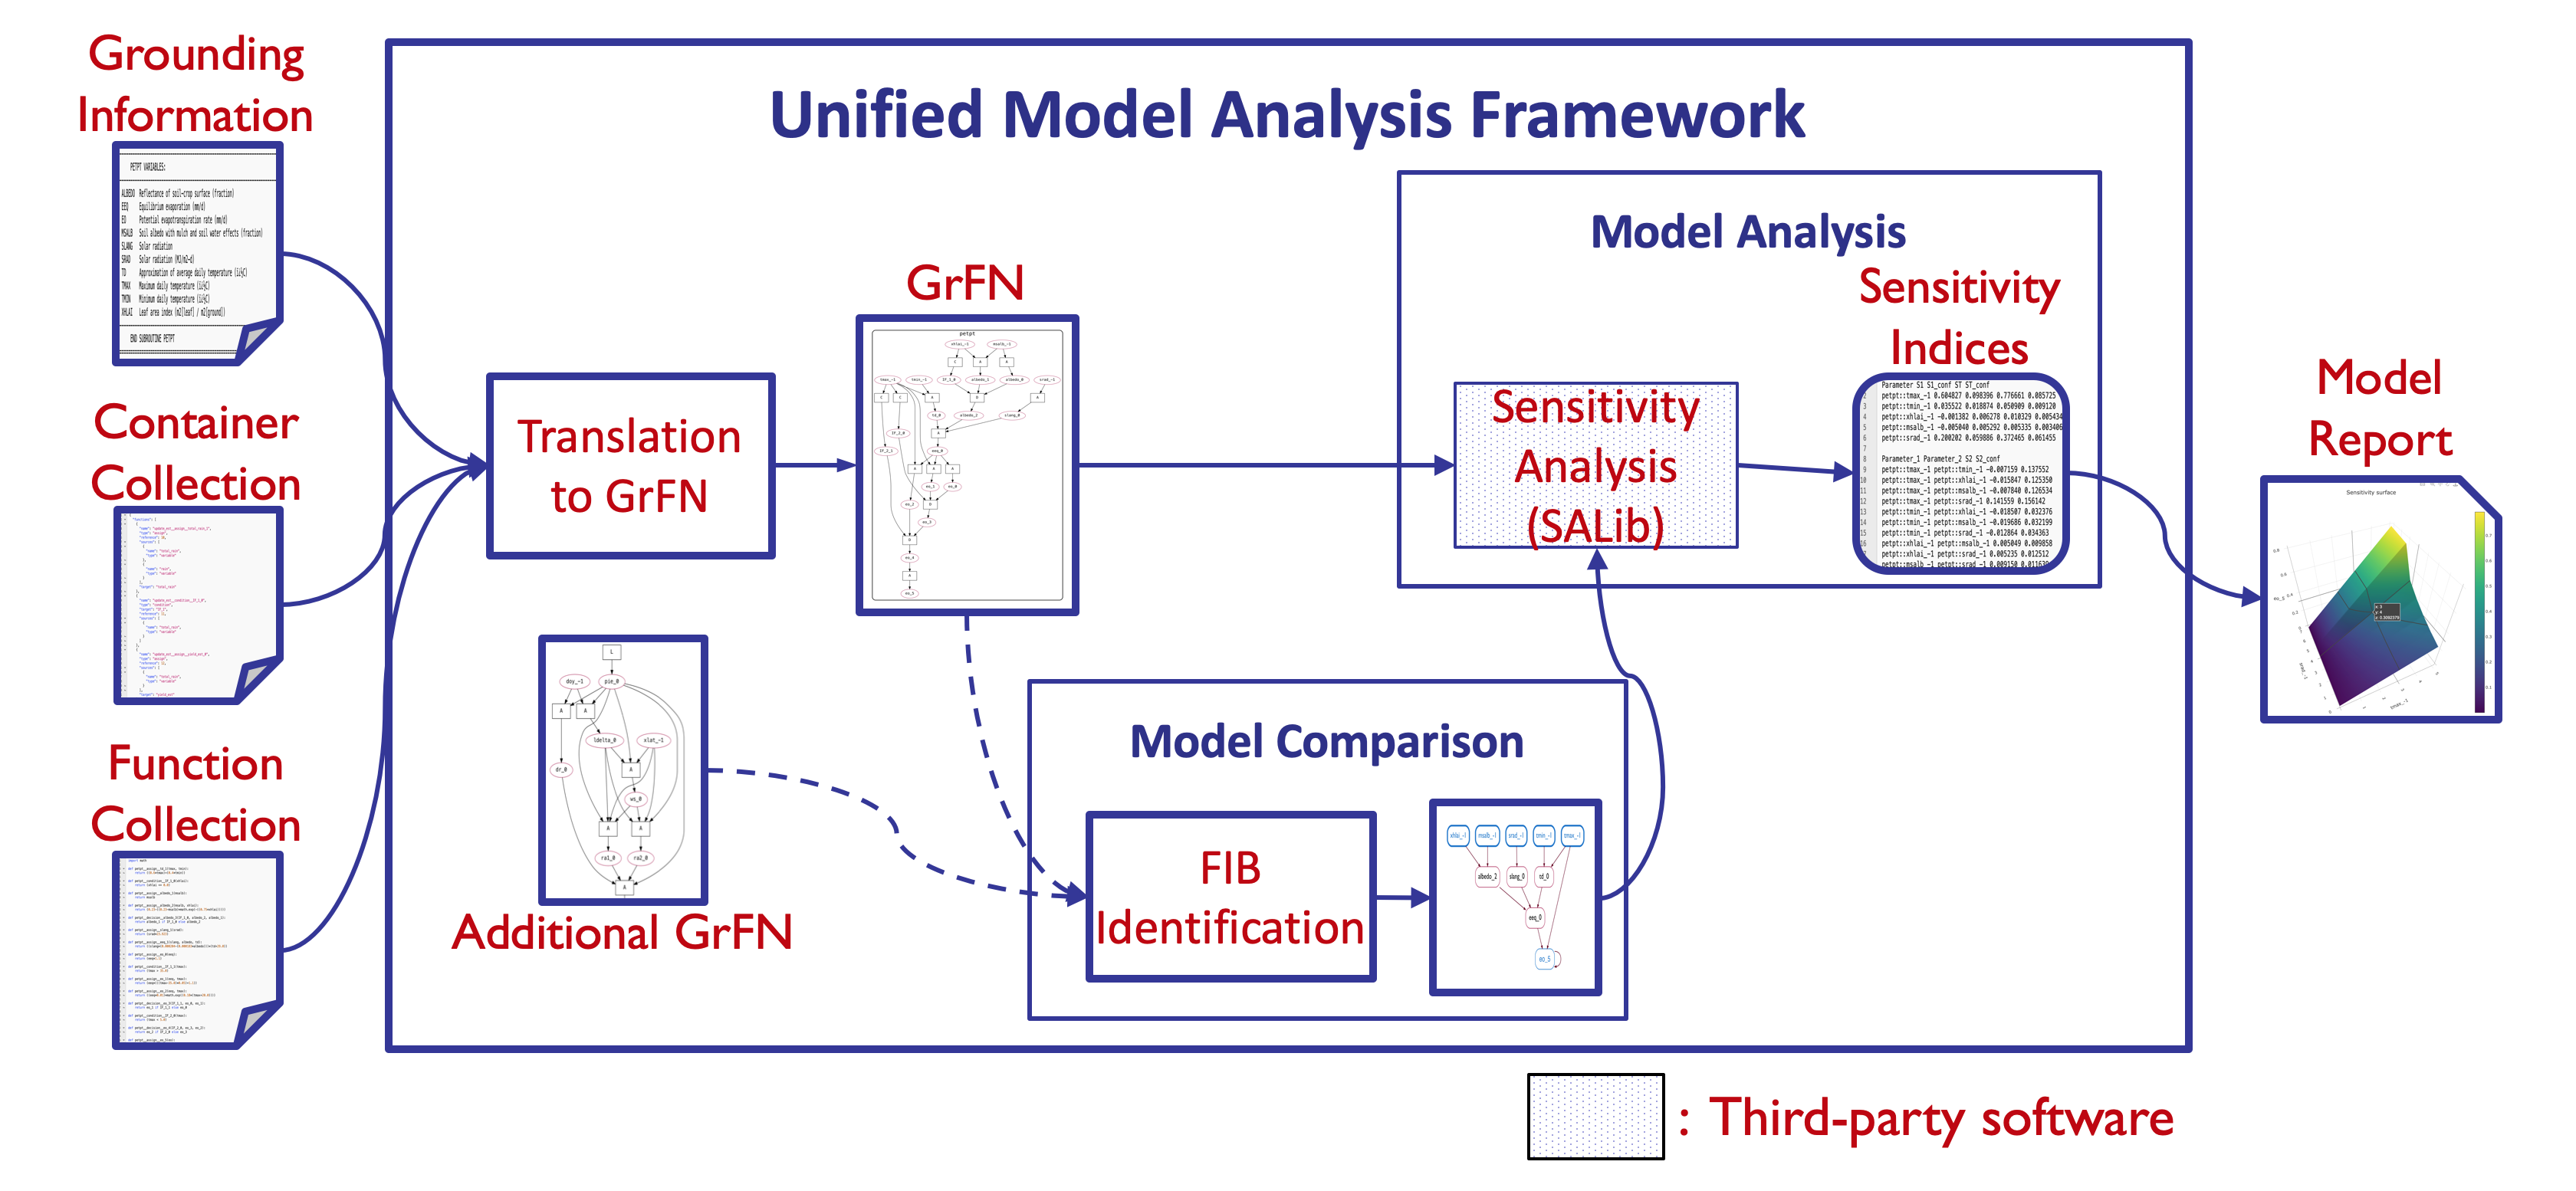
\includegraphics[width=\columnwidth]{UMAF}%
    \caption[Diagram of UMAF]{This figure shows the entirety of the UMAF framework. We see that the framework takes in a function collection, container collection, and variable grounding information from the original source code program and then converts these inputs into a GrFN. The GrFN can then be used for model comparison and analysis, and the results of these processes are packaged into a model report.}
\end{figure}

\section{UMAF Inputs from the AutoMATES Pipeline\label{sec:umaf_inputs}}
In this section I will provide a brief overview of the current state of the modules in the AutoMATES pipeline whose outputs serve as input to UMAF.
The three modules that provide inputs to UMAF are \textit{Program Analysis} (PA), \textit{Text Reading} (TR), and \textit{Equation Reading} (ER). As seen in Fig~\ref{fig:automates_pipeline}, the PA module takes a Fortran program as its input and produces an abstract syntax tree of the scientific model portion of the program as its output.
The TR module reads both associated texts from the scientific literature for a particular source code model and the documentation found in source code for that model.
From these texts the TR module extracts useful information that can be used to link the variables in source code to the real-world values they represent.
The ER module module can also be used to facilitate this linking process.
The ER module uses images extracted from publications related to the source code models to reconstruct the mathematical equations present in the images.
These equations can then be linked to mathematical equations extracted from source code in order to assist in linking source code variables to descriptions of variables found in an equation that was present in a publication.
This process is especially necessary when documentation for the variables found in source code is either missing or incomplete.
In the following subsections I will briefly describe the methods used by each of these modules in order to obtain the outputs required by UMAF.

\subsection{Overview of the Program Analysis Pipeline\label{sec:pa_overview}}
In order for UMAF to create a GrFN from source code it requires the source code to be transformed into a representation that captures the computations required to compute the variables contained in a source code program and the wiring of variables in the source code program.
In order to fulfill both of these requests the PA module performs a translation from the original source code into two components, a \textit{function collection} that stores the computations required to compute each variable and a \textit{container collection} that records what variables are used in each statement of each code container of the original source program.
UMAF will be able to use these two components in order to produce the function network component of a GrFN that explicitly represents the wiring among variables in the GrFN while providing access to inspect the computations used to compute each variable.
An added component of the functionality of the PA module is to translate the source code programs from their initial programming language into a single intermediate representation language that can be read by UMAF.
This allows for UMAF to focus on translating a single input source (namely the statement list produced by the PA module) as opposed to needing to be able to translate all of the many programming languages and idioms into GrFN.
Currently the PA module only translates Fortran programs into the intermediate representation; however, as a component of AutoMATES the PA module is intended to translate models written in other languages and programming styles during the lifespan of the project.

The process conducted by the PA module to translate the Fortran source code for a scientific model starts by using the Open Fortran Parser (OFP) \footnote{\url{https://github.com/OpenFortranProject/open-fortran-parser}} in order to extract an abstract syntax tree (AST) \citep{aho1986dragonBook} from the original source code.
The AST form of the program provides a language-agnostic view of the components of the program that can be a common target for many different source code languages as their first step in the the PA module translation.
the PA module will then take advantage of the AST structure to identify containers of portions of code, such as loops and function calls.
Other containers can exist in the original source code, such as unconditional branching and looping containers created by \texttt{goto} statements.
A preprocessing step in the the PA module system is to translate all unstructured containers into a structured variant that tracks input variables into the container and the output variables expected from the container.
This is necessary in order to complete the variable wiring for a GrFN across the containers found in the original source code.
Under each container exists an ordered list of statements.
Statement are either assignment statements or conditional statements, both of which will produce variables that need to be wired into a GrFN and include a computation that details how the variable is produced as a product of other variables.

Assignment statements represented in an AST will have an explicit variable being assigned and a computation used to perform the assignment.
This form easily allows the PA module to extract the computation that will be separated as a \textit{black-box} function, associated with the variable being assigned, and added to the function collection.
With a minor amount of inspection, the PA module will then determine what variables are used in the computation that need to be wired to the assignment variable as inputs and will then add an entry to the containers statement list in the container collection.
While multiple assignment statements to the same variable can occur in a program, GrFN is concerned with the flow of data through the scientific model represented by a program.
Thus the PA module performs the additional task when translating an assignment statement of indexing updates to variables with the same name to preserve the flow of data for the wiring step of GrFN creation.
In an imperative programming language, conditional statements involve both control-flow actions and data-flow actions.
the PA module handles conditional statements by splitting the statement into a condition evaluation that regulates control flow through the conditional, and a set of decision statements, one per assignment statement found under the conditional that determines the flow of data to the variable assigned under the conditional.
The computations and wiring required for the condition and decision statements are handled similarly to the assignment statement described above and added to the function collection and statement list of the container collection respectively.
Once all containers of the original program have been processed, the function collection and container collection are ready to be sent to UMAF, where they will be translated into GrFN.

\subsection{Overview of the Text and Equation Reading Modules \label{sec:ter_overview}}
While the PA module is able to provide all of the wiring needed to create a function network and the computations needed to make the network executable, UMAF requires additional inputs in order to perform the variable grounding necessary to create a GrFN.
These inputs come from the TR Module and the ER Module.
The information we are interested in gathering from these two modules is a mapping of variables mentioned in the program source code to real-world concepts present in the system being modeled.
In order to perform the mapping, the TR module makes use of text information from publications associated with the scientific models, as well as variable documentation present in the source code.
The TR module will first extract possible variables from the associated publications using the ODIN \footnote{\url{https://github.com/clulab/processors/wiki/ODIN-(Open-Domain-INformer)}} event extraction framework \citep{valenzuela2015Odin}.
During the extraction process each of variable will have a text portion associated with it that has been determined to be a description of the variable from the publication.
An example of extracting variables with associated descriptions is shown in Fig~\ref{fig:odin_extraction_example}.
The TR module can perform the mapping by computing a word-overlap score between the text description of each of the possible variables from the associated publication with the variable documentation snippets found in the source code.
Descriptions that have high enough overlap are then linked and the variables present in the source code that correspond to the documentation snippet are considered grounded to the variable extracted from the associated publication.

\begin{figure}[!htbp]
    \label{fig:odin_extraction_example}
    \centering
    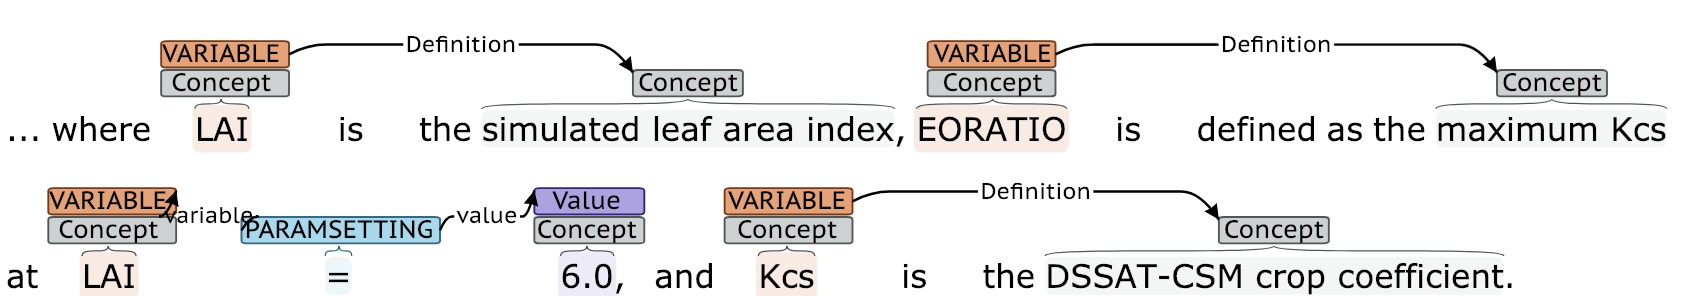
\includegraphics[width=.8\columnwidth]{TR_Odin_extraction_rules}%
    \caption[Example Variable Extraction via ODIN]{An example of variables and associated text descriptions being extracted by the ODIN rule-based extraction framework.}
\end{figure}

However, sometimes documentation snippets do not exist for the variables found in source code, or the documentation could be incomplete.
In these cases the ER module can be used to help determine how to correctly ground variables to those found in the associated publication.
The ER module works by transforming images of equations found in the associated publication into a programmatic structure of the computation defined by the equation.
This structure can then be linked to the similar computation contained in the source code, thus linking the computation to the equation in the associated publication.
Once this is accomplished the variables in the computation will be linked to symbols in the initial equation.
At that point the TR module can link descriptions of variables found in the publication text to the symbols found in the equation.
With this final linking, the variables in the source code can now be transitively grounded to the descriptions of variables found in text, without ever requiring documentation about the variables to be present in the source code.
Using these two modules allows for the majority of variables present in the source code representation of a scientific model to be linked to real-world phenomena, and will give UMAF the information necessary to ground the wiring of the function networks to produce GrFNs that satisfy the condition of being comparable.

\section{Constructing a Grounded Function Network \label{sec:grfn_assembly}}
The goal of UMAF is to transform the inputs from the PA, TR, and ER modules into a GrFN.
The first step of this process is to create the function network from the inputs provided by the PA module.
This process involves a translation step from the imperative representation of a program that is extracted by the PA module to a dataflow representation that can be naturally represented as a function network.
During the creation of the function network, variables contained in it can be grounded using the outputs from the TR and ER modules.
The second step required to construct a GrFN is to extract the GrFN execution stack from the function network so that the GrFN can be executed efficiently.
In this section I will begin with an explanation of both of the steps required to create an executable GrFN.
Afterwards I will demonstrate an example of the translation process from the original program source code to an executable GrFN.

\subsection{Translation to a Function Network \label{sec:trans_to_dfm}}
Most programs are written in languages that follow the von Neumann vision of sequential instruction execution.
This means that programs are defined as a list of instructions that are executed in the sequential order that they are written.
This representation and execution style is unnatural for a scientific model because models need not be expressed sequentially.
It is certainly the case that some computations in a scientific model must occur after others; however, there need not be a total ordering upon the computations included in the scientific model.
The only necessary restriction for executing a scientific model is that all of the inputs for a given function must populate with values before the function can be evaluated.
This execution style pairs well with programs that are written using the dataflow programming idiom \citep{johnston2004dataflowadvances}.
While traditional programming idioms, such as imperative programming, represent a program as a sequential list of instructions that are executed in a pre-defined order, dataflow programs are represented as a series of connections between inputs and outputs with connecting operations between them that function as black-box computations \citep{wadge1985lucid}.
This is the exact same specification as we have required for the function network component of a GrFN, and thus a GrFN is a representation of a dataflow program.
Therefore the process of creating a GrFN from the inputs provided to UMAF can be reduced to the process of translating an imperative representation of a program to a dataflow representation of a program, and then grounding the variables present in the new dataflow program.

While imperative programs are easily expressed as lines of code in flat files, this expression format is unnatural for a dataflow program.
A dataflow program, such as the GrFN created by UMAF are much more naturally expressed as networks.
A \emph{network} is a directed acyclic graph that contains a set of source nodes and a set of sink nodes \citep{bondy1976graph}.
A node is considered a source node if the in-degree of the node, the number of directed edges arriving at the node is zero.
Similarly a node is considered a sink node if the out-degree of the node, the number of directed edges leaving the node, is zero.
The networks used to construct a GrFN are function networks, meaning the network will include two types of nodes, variable nodes and function nodes.
This network will be bipartite upon the set of variable nodes and the set of function nodes.
This entails that no function node has an edge incident to another function node, and no variable node has an edge incident to another variable node.
Since GrFN is intended to represent a scientific model, the source variable nodes of the GrFN will be the model inputs, and the sink node represent the model output.

The function network for a GrFN is created by performing a recursive traversal through each container of the container collection passed in to UMAF by the PA module.
Translating a container into the function network involves:
\begin{enumerate}
  \item Unify inputs to the container from its parent container, with the names used for the inputs in the containers statement list.
  \item Process the containers statement list one line at a time.
  \begin{enumerate}
    \item If the line is a call to a new container:
    \begin{enumerate}
      \item Create a new plate in the function network that will contain all of the nodes created by this container.
      \item Setup the container inputs
      \item Recurse to and process the child container
      \item Unify outputs from the child container with the current variables.
    \end{enumerate}
    \item Otherwise if the statement is an \texttt{assignment}, \texttt{condition}, or \texttt{decision} statement perform the following operations:
    \begin{enumerate}
      \item Generate a new function node containing the computation associated with the statement.
      \item Create new variable nodes for each input recorded for the statement as well as the statements output.
      \item Wire the inputs with directed arcs to the new function nodes
      \item Wire a directed arc from the new function node to the output node
    \end{enumerate}
  \end{enumerate}
  \item Prepare a collection of all of the outputs from the container. This is likely a mixture of container return values and updated variables whose scope survives the scope of the container.
  \item Back out to the parent contained with the output variable set, or return the completed network if at the root container.
\end{enumerate}

\begin{figure}[!htbp]
  \label{fig:grfn_cgs}
  \centering
  \subfloat[PETPT GrFN]{
    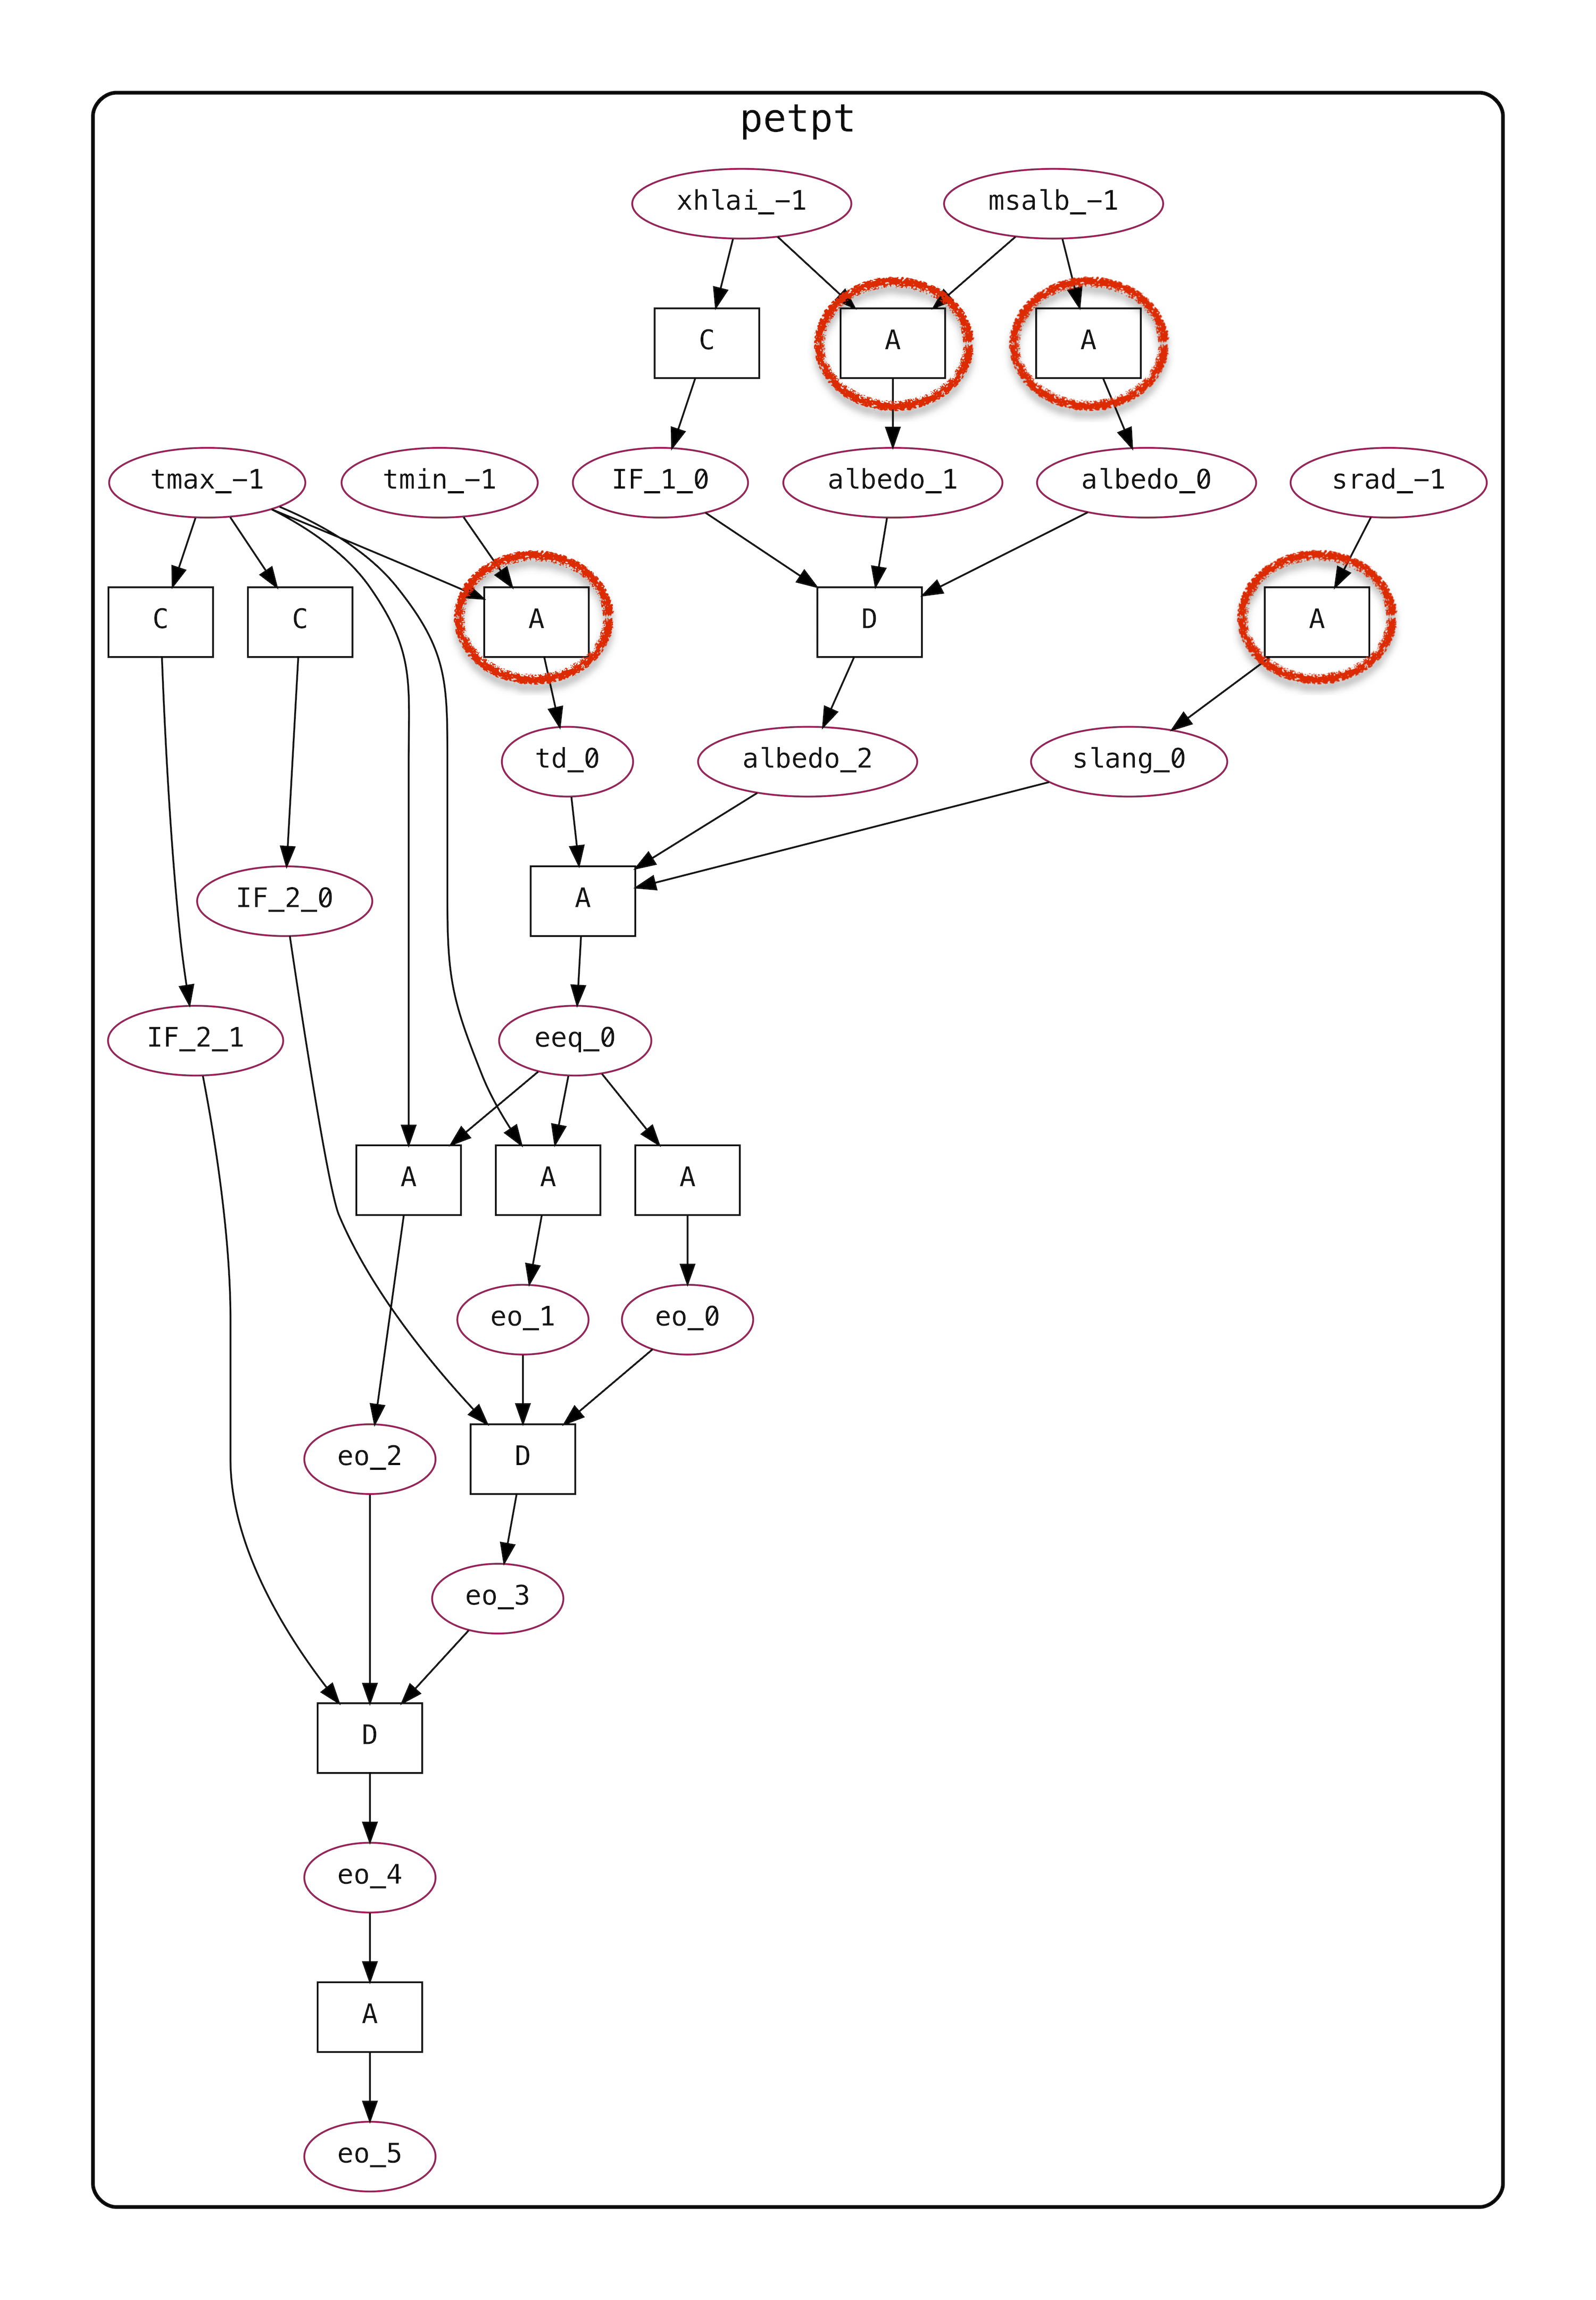
\includegraphics[width=0.45\textwidth]{PETPT_GrFN_smaller}
    \label{fig:petpt_grfn_cg}
  }
  \hfill
  \subfloat[PETASCE GrFN]{
    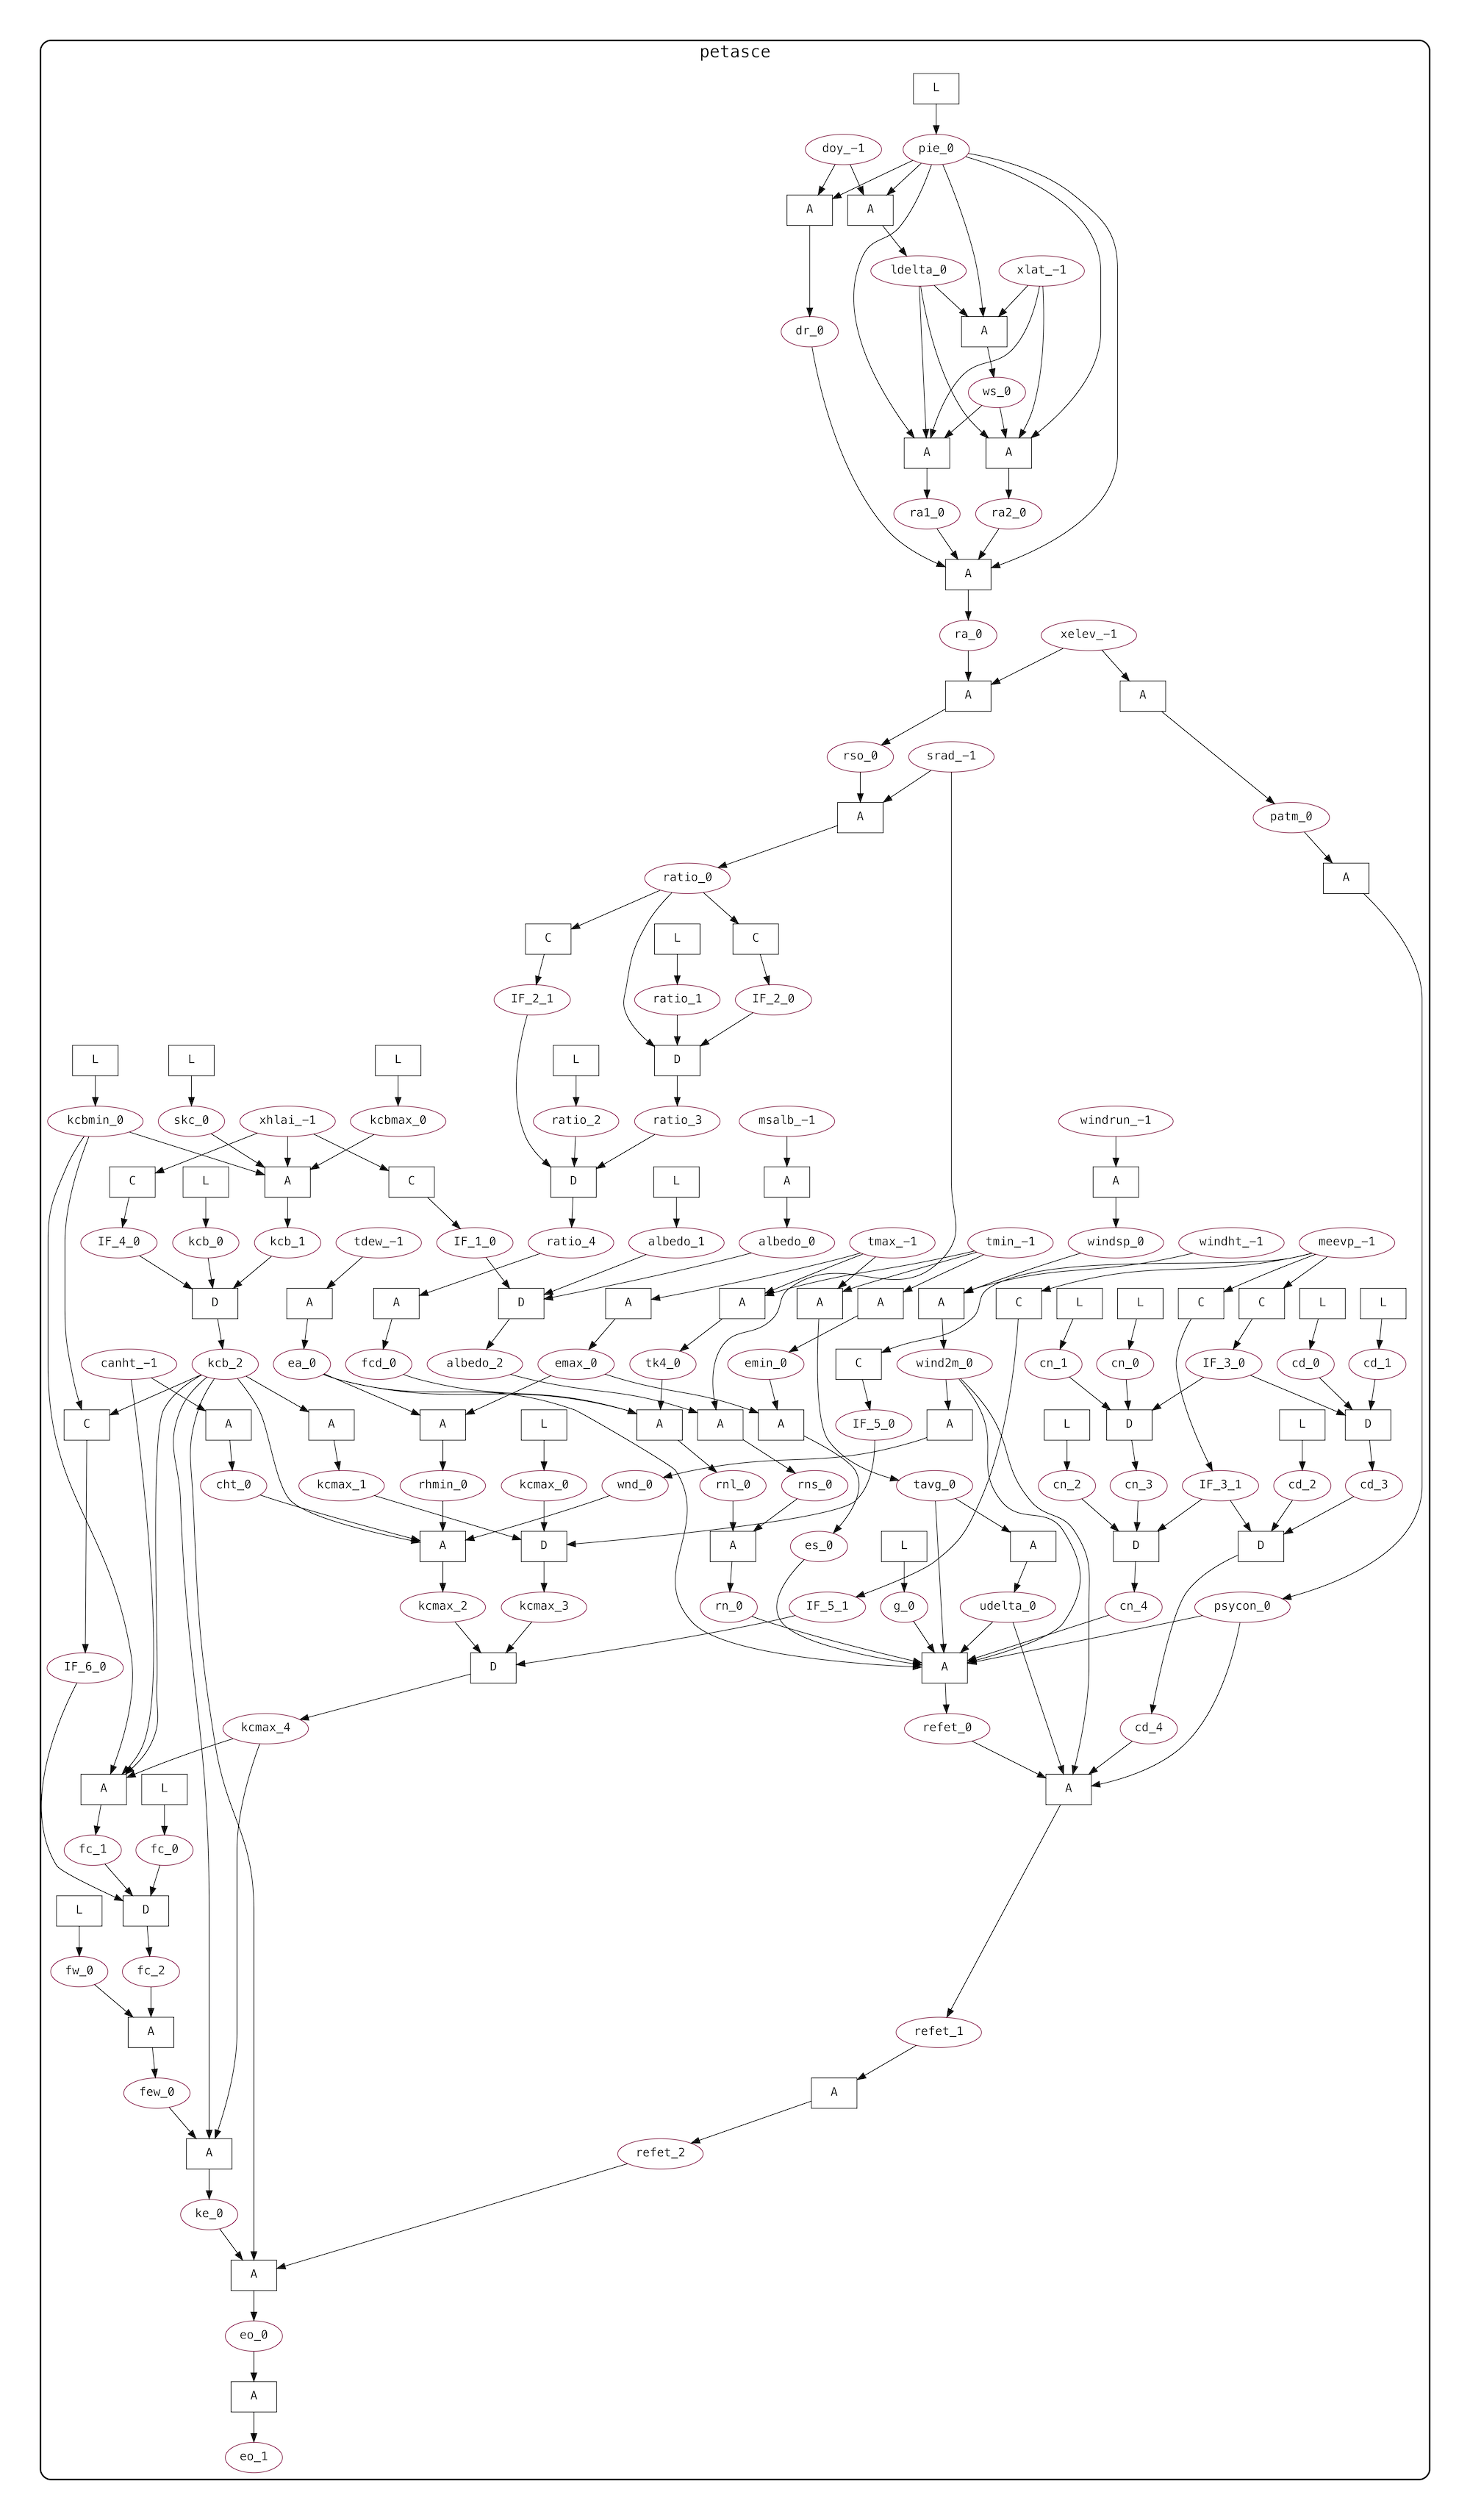
\includegraphics[width=0.45\textwidth]{PETASCE_GrFN_smaller}
    \label{fig:petasce_grfn_cg}
  }
  \caption[Evapo-transpiration GrFN Examples]{GrFNs for the PETPT and PETASCE evapo-transpiration modules. The visual representations include the variables, represented as circle nodes, with names derived from the names extracted in the source code and variable name grounding inference; the variable names also include a numeric index representing variable state changes during processing (see text for further details). Function nodes are depicted as squares with a single letter representing the type of function contained at the node. Function types include: assignment (A), conditional (C), decision (D), or literal (L).}
\end{figure}

The process described above will generate a function network to serve as the basis for a GrFN.
The only additional processing left to create a GrFN is to complete a traversal of the function network in order to visit every variable node, and to ground the variable nodes that have been linked using the inputs from the TR and ER modules.
Once the traversal is complete the translation to GrFN has been completed.
Figure~\ref{fig:grfn_cgs} shows two completed GrFNs one for the ASCE model and one for the Priestley Taylor model of potential evapo-transpiration.
These GrFNs were translated from the actual Fortran source code for these two models from the DSSAT code base, both of which are available in Appendix~\ref{appendix:a}.

\subsection{Extracting a GrFN Execution Stack \label{sec:exec_graph_extraction}}
Creating a GrFN allows us to formally represent a scientific model from source code as a dataflow program.
However, if we wish to analyze the GrFN, then we will need the ability to execute GrFNs given a set of input values.
A GrFN can be executed by executing the lambda functions stored in all of the function nodes.
As stated in the previous subsection, the function nodes rely upon having values populated at each of their input variable nodes in order to execute their lambda functions.
Therefore, if an ordering is defined over the execution of the function nodes contained in a GrFN that ensures that no function node is executed before values populate to the node, then the GrFN will be able to execute correctly.

A Naïve first-pass solution to accomplish this goal would be to use a graph traversal from the output to the inputs where at each function node, the node will determine whether values for each input variable node have been populated.
For any input variable nodes that have not been populated, the function node will call the parent function node responsible for computing the value of the input variable node.
Once all such calls have returned, the function itself will evaluate. This recursive calling procedure is very similar to message-passing, a method for inference on factor graphs \citep{bishop2006pattern}.
While this will ensure correct model execution, this method of handling execution is not as efficient as possible.
Two obvious inefficiencies are that the recursive call structure requires additional function setup and calls to the execution, on the order of the number of functions included in the computation graph, and this execution style requires recursive message passing for each execution.

% NOTE: Pickup revisions here
These two concerns can be addressed by creating a call stack comprised of all the function nodes contained in the GrFN CG.
The order of computation between function nodes implies that the call stack is equivalent to a partially ordered set (poset) upon the function nodes \citep{simovici2008miningTools}.
Once this poset is recovered, execution of the GrFN CG can occur by executing all functions at the first level in the poset, then moving to the next level in the poset, and then repeating the sequence until reaching the end of the call stack.
This allows all function nodes at the same level in the poset to be executed concurrently, and the computation required to create this call stack only needs to occur once.

Computing the call stack requires a series of separate computations.
First a network flow graph (NFG) \citep{allen1970CFG} must be extracted from the GrFN.
As defined above, the GrFN CG is bipartite with respect to the variable and function nodes, such that no variable node is adjacent to another variable node and vice-versa for a function node \citep{bondy1976graph}.
Therefore a GrFN NFG can be extracted from the GrFN CG by simply squashing any variable node between a pair of function nodes into a singular edge connecting the two function nodes.

\begin{figure}[!htbp]
    \label{fig:petpt_nfg}
    \centering
    \includegraphics[width=\columnwidth]{PETPT_GrFN_NFG}%
    \caption[PETPT GrFN Network Flow Graph]{This figure is a visualization of the Network Flow Graph (NFG) for the PETPT model. The nodes in this graph represent function nodes in the PETPT GrFN and connections between nodes represent the flow of data through the function nodes in the PETPT GrFN.}
\end{figure}



Since the GrFN NFG is derived from the GrFN CG it will have a set of input nodes.
Starting from this set of input nodes an index is assigned to each node, beginning at zero.
Each time an edge is traversed the index increases.
If a function node is reached and it already has an index the index is updated to the maximum of the current index and the newly calculated index.
Once the full graph traversal is complete we have an index for the poset.
Function node sets are created according to the index values, and the index values also provide the ordering of the function node sets.
Smaller index values correspond to the function node sets that are to be computed first.
Function sets can then be placed into the call stack by pushing the sets with the largest index value onto the stack first.
The GrFN CG now has access to a call stack that can be used to execute an input set.
During execution, when the call stack is being used, it can be maintained by pushing popped values from the stack onto a different empty stack.
After execution, the values can be popped from the temporary stack and pushed back on to the original call stack.
This ensures that the call stack order will be maintained for the next execution.

\begin{figure}[!htbp]
  \label{fig:petpt_execution_stack}
  \centering
  \begin{tikzpicture}[stack/.style={rectangle split, rectangle split parts=#1,draw, anchor=center}]
    \node[stack=7, text width=15cm, align=center]  {
      \nodepart{one} \texttt{petpt\_\_condition\_\_IF\_1\_0, petpt\_\_assign\_\_albedo\_0}, \\
      \texttt{petpt\_\_assign\_\_albedo\_1, petpt\_\_assign\_\_td\_0}, \\
      \textt{petpt\_\_assign\_\_slang\_0},
      \texttt{petpt\_\_condition\_\_IF\_2\_0}, \\
      \texttt{petpt\_\_condition\_\_IF\_2\_1}
      \nodepart{two}\texttt{petpt\_\_decision\_\_albedo\_2}
      \nodepart{three}\texttt{petpt\_\_assign\_\_eeq\_0}
      \nodepart{four}\texttt{petpt\_\_assign\_\_eo\_0}, \texttt{petpt\_\_assign\_\_eo\_1}, \\ \texttt{petpt\_\_assign\_\_eo\_2}
      \nodepart{five}\texttt{petpt\_\_decision\_\_eo\_3}
      \nodepart{six}\texttt{petpt\_\_decision\_\_eo\_4}
      \nodepart{seven}\texttt{petpt\_\_assign\_\_eo\_5}
    };
  \end{tikzpicture}
  \caption[PETPT GrFN Execution Stack]{This figure shows the execution stack partial ordering for the PETPT GrFN model. The names present in the stack correspond to function nodes that are showed in PETPT's NFG diagram in Fig~\ref{fig:petpt_nfg}. Executing all of the function nodes at each stack level in order will complete the execution process for the PETPT GrFN.}
\end{figure}

During execution, a GrFN utilizes a value storage tag at each variable node.
During computation, function nodes pull their input data from the value tag of each parent variable node of the function node.
The output from the function node is stored in the value tag of the variable node that is the child of the function node.
The partial ordering upon the execution stack guarantees that function nodes have access to the variable node input data at the time of their execution.
After all function nodes have been executed the output variable node of the GrFN CG will have the computed output value stored in its value tag.


\subsection{Data Type Assignment\label{sec:data_type_assg}}
% TODO: revise the content in this section
So far I have discussed the wiring needed to create the computation graph that will allow a GrFN to be executed, and I have shown the methods necessary to make the GrFN executable.
However, one more crucial component for creating a GrFN that we can perform inference upon is a discussion of how we will handle the actual data being processed from the GrFN.
At the time of writing this thesis only basic data types are allowable in a GrFN. This includes numerical, string, and boolean values.
These primitive data types are all singular values that represent a single phenomena, thus they match perfectly with the definition of variable nodes in the GrFN CG.
The specification for each variable in a GrFN CG contains a type annotation that declares the data type of the variable.
These values are derived from the JSON specification during the wiring stage of the GrFN.
At execution time, these type annotations are used to validate a set of inputs and ensure proper storage format of computed variable values.

The infrastructure to represent complex data types such as Arrays, user-defined types, and unions in the AST form is still being developed by the program analysis team, and thus they will not be included in this thesis.
The main challenge with representing these data types is that they are not singular variables, but are instead collections of variables.
To properly perform inference over a GrFN CG all variable nodes must be singular variables, thus we cannot allow any of the above collections of variables to be represented by a variable node.
This presents a problem of representation that will be studied  and resolved in future work that extends this thesis.




\subsection{Source Code to Computation Graph Example\label{sec:code_to_grfn}}
To illustrate the process of constructing an executable computation graph from source code, consider the toy model for crop yield example from Figure~\ref{fig:simple_crop_CAG}.
The Fortran code for this model is shown in Figure~\ref{fig:crop_code} below.

\begin{figure}[!htbp]
    \label{fig:crop_code}
    \centering
    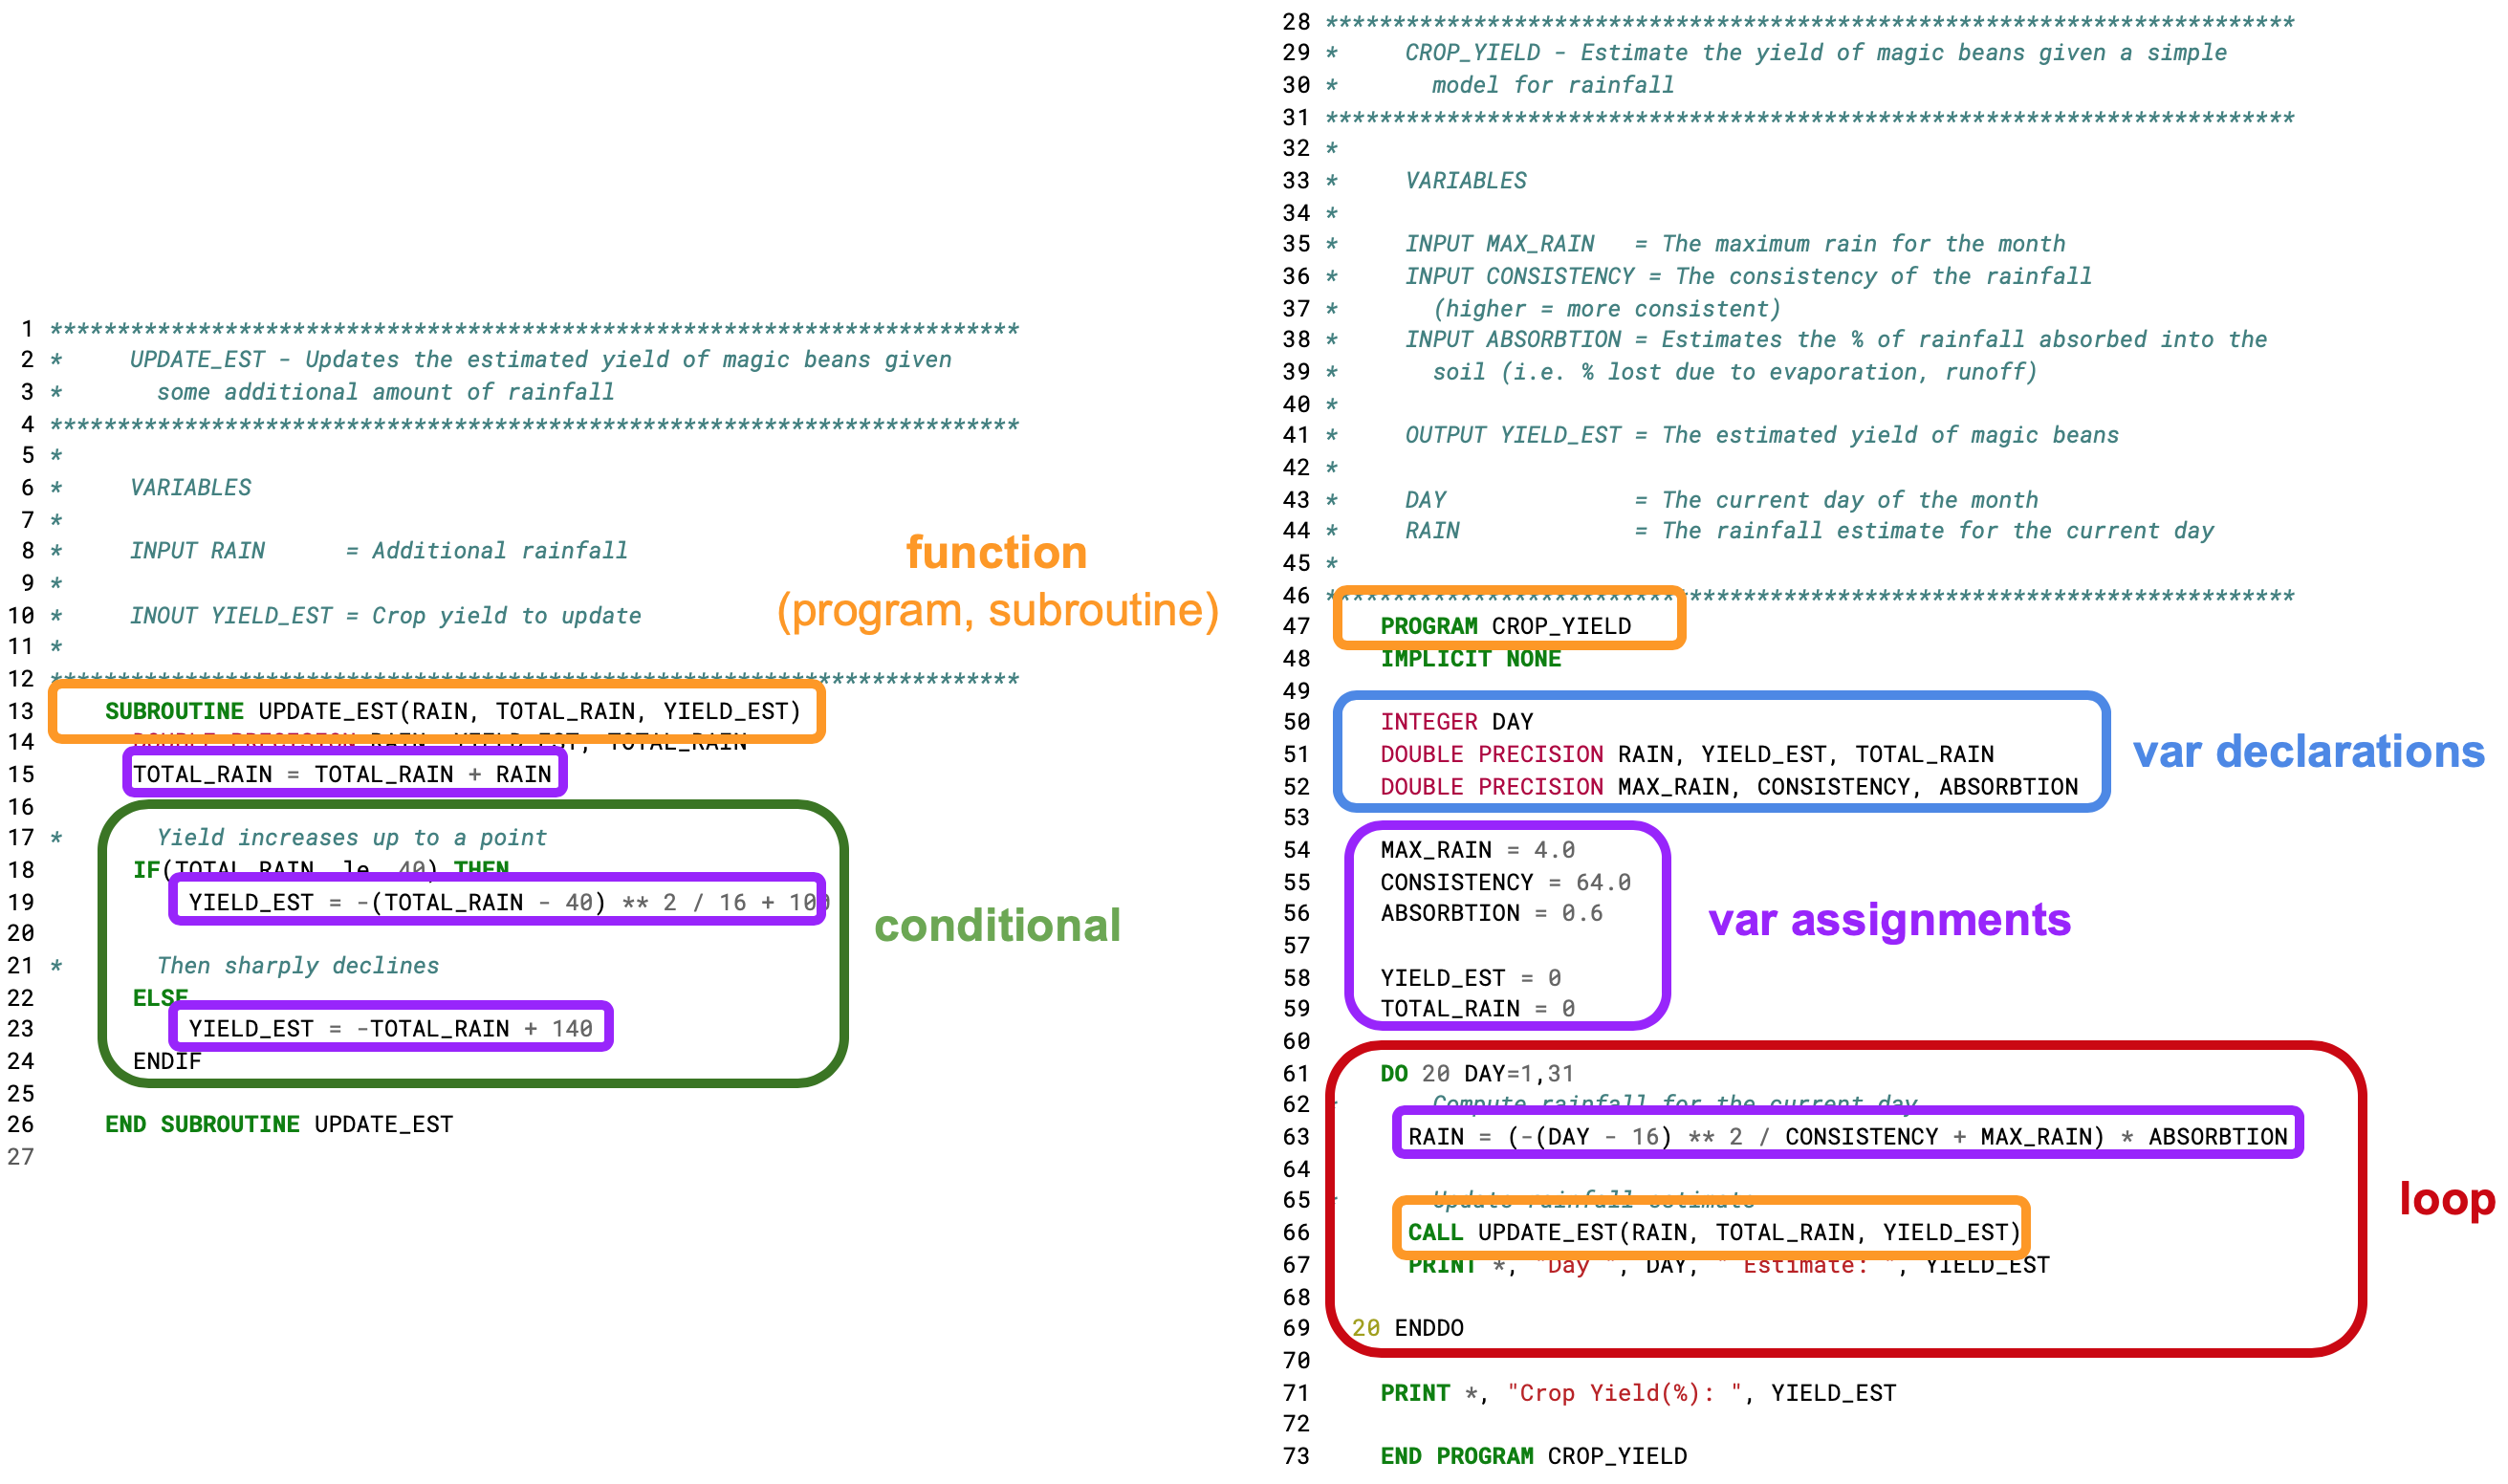
\includegraphics[width=\columnwidth]{CROP_YIELD_CODE}%
    \caption[Crop Yield Model Source Code]{Fortran source code for the toy model of Crop Yield.}
\end{figure}

From inspecting the source code we see that this model has many programming idioms that need to be handled in order to create an executable computation graph for the source code.
As noted in the figure this includes subroutines, conditional statements, variable declarations, assignment statements, as well as loops.
The SMS pipeline handles all of these idioms and is able to produce the following executable computation graph, shown in Figure~\ref{fig:crop_grfn_cg} below, that is faithful to the structure of the model found in the source code. In the following section I will delve into the specifics of how the SMS pipeline is able to create an executable computation graph from a source code representation.

\begin{figure}[!htbp]
    \label{fig:crop_grfn_cg}
    \centering
    \includegraphics[width=\columnwidth]{CROP_YIELD_GrFN}%
    \caption[Crop Yield Model GrFN CG]{Executable computation graph for the toy Crop Yield model.}
\end{figure}


\section{GrFNs are Dynamic Bayes Nets\label{sec:grfn_as_dbn}}
% TODO: finish revising this section
Once we have extracted a GrFN CG that represents a scientific model we will want to analyze the model and compare it to other existing models.
Both of these tasks require us to be able to perform inference on the GrFN CG by observing the behavior of the model over a distribution of inputs.
A well defined methodology for performing inference over DAGs is to establish the DAG as a bayesian network \citep{bishop2006pattern}, a type of probabilistic graphical model, and then to use the robust set of methods associated with bayes nets to solve inference problems.
In this section I will now demonstrate how a GrFN CG is a bayesian network in order to unlock the use of inference on GrFN CGs.

A GrFN CG has a set of input variables that are wired as a network to the outputs of the model represented by the GrFN CG.
The inputs of the GrFN CG can be assigned values and will then return an output value for each of the GrFN CG outputs.
Recall that all variables in a GrFN CG are treated as random variables.
Bayes nets have a set of variables that are linked to observable random variables that exist in the real world.
This presents a challenge for representing a GrFN CG as a bayes net because several variables in a GrFN CG represent the same natural phenomena.
However, we can view a GrFN CG as a \emph{Causal Analysis Graph} (CAG) that allows us to visualize only the variable relationships present in the GrFN.
Below are the CAG views for the two GrFN CGs under study in this thesis. Notice that inspecting this view gives us a graph structure that looks similar to a bayes network that has loops (i.e. one that can be unrolled over time).

\FloatBarrier
\begin{figure}[!tbp]
  \centering
  \subfloat[PETPT GrFN CAG]{
    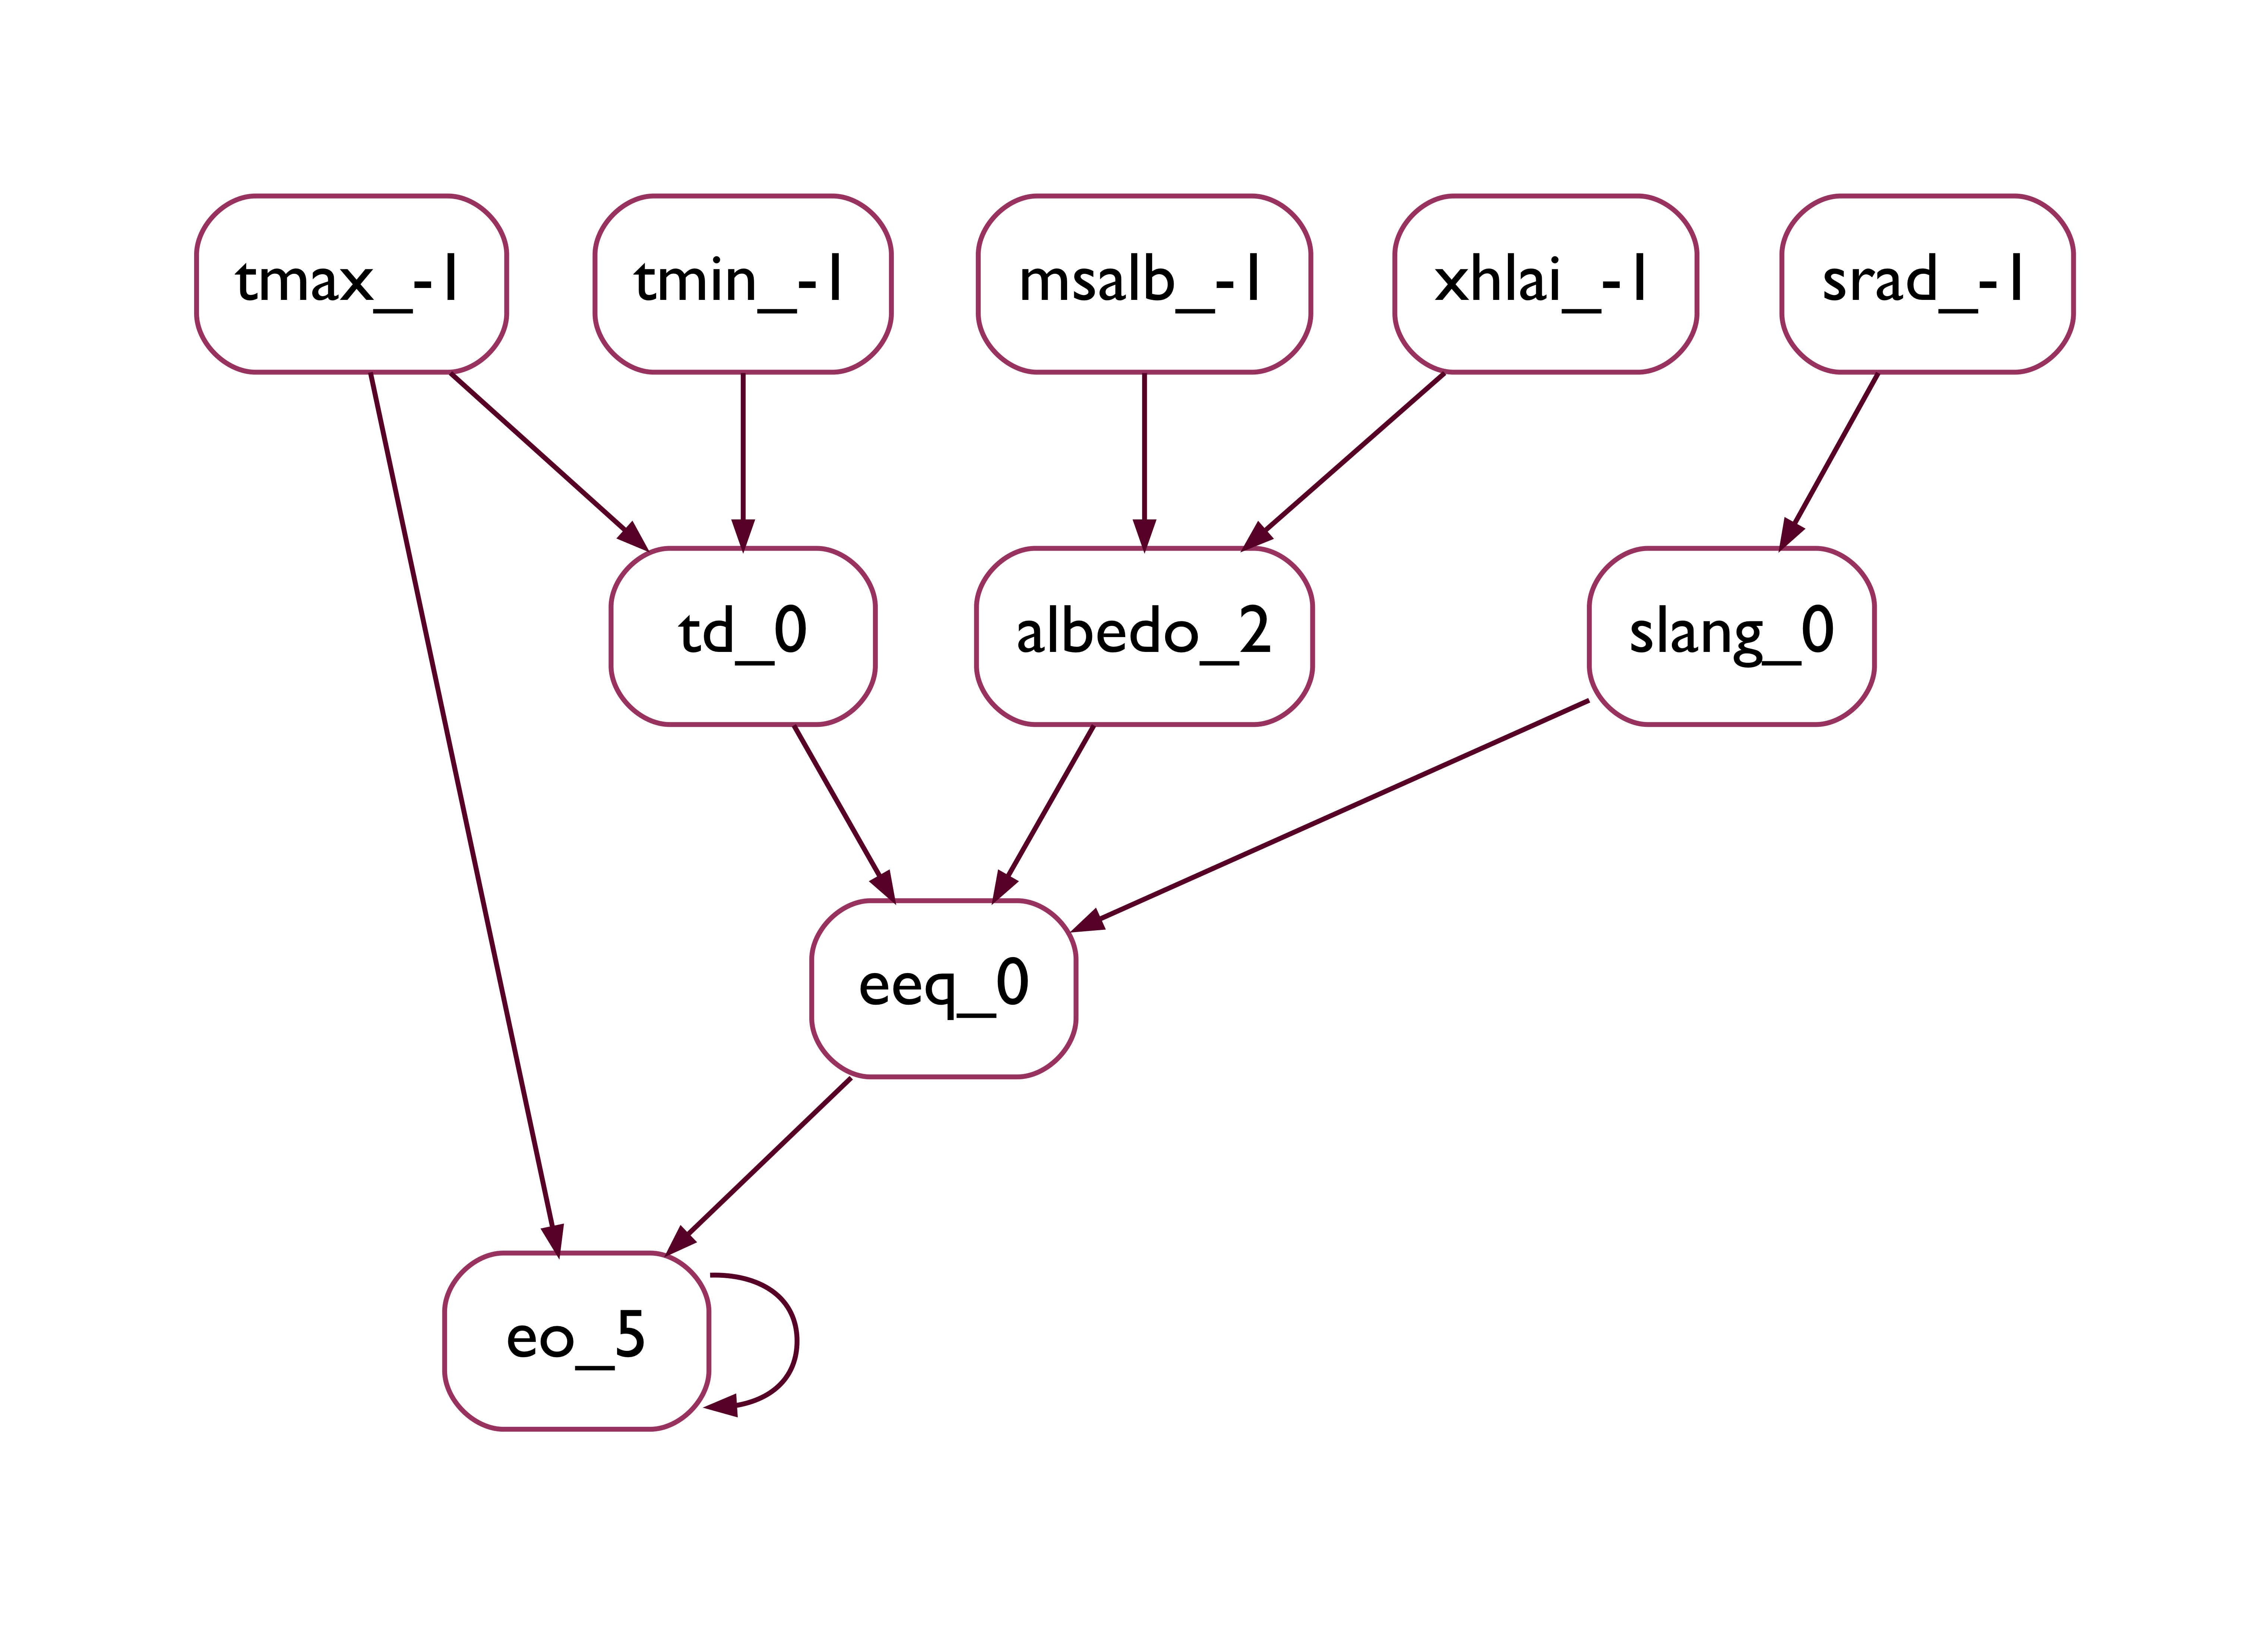
\includegraphics[width=0.75\textwidth]{PETPT_GrFN_CAG}
    \label{fig:petpt_cag}
  }

  \subfloat[PETASCE GrFN CAG]{
    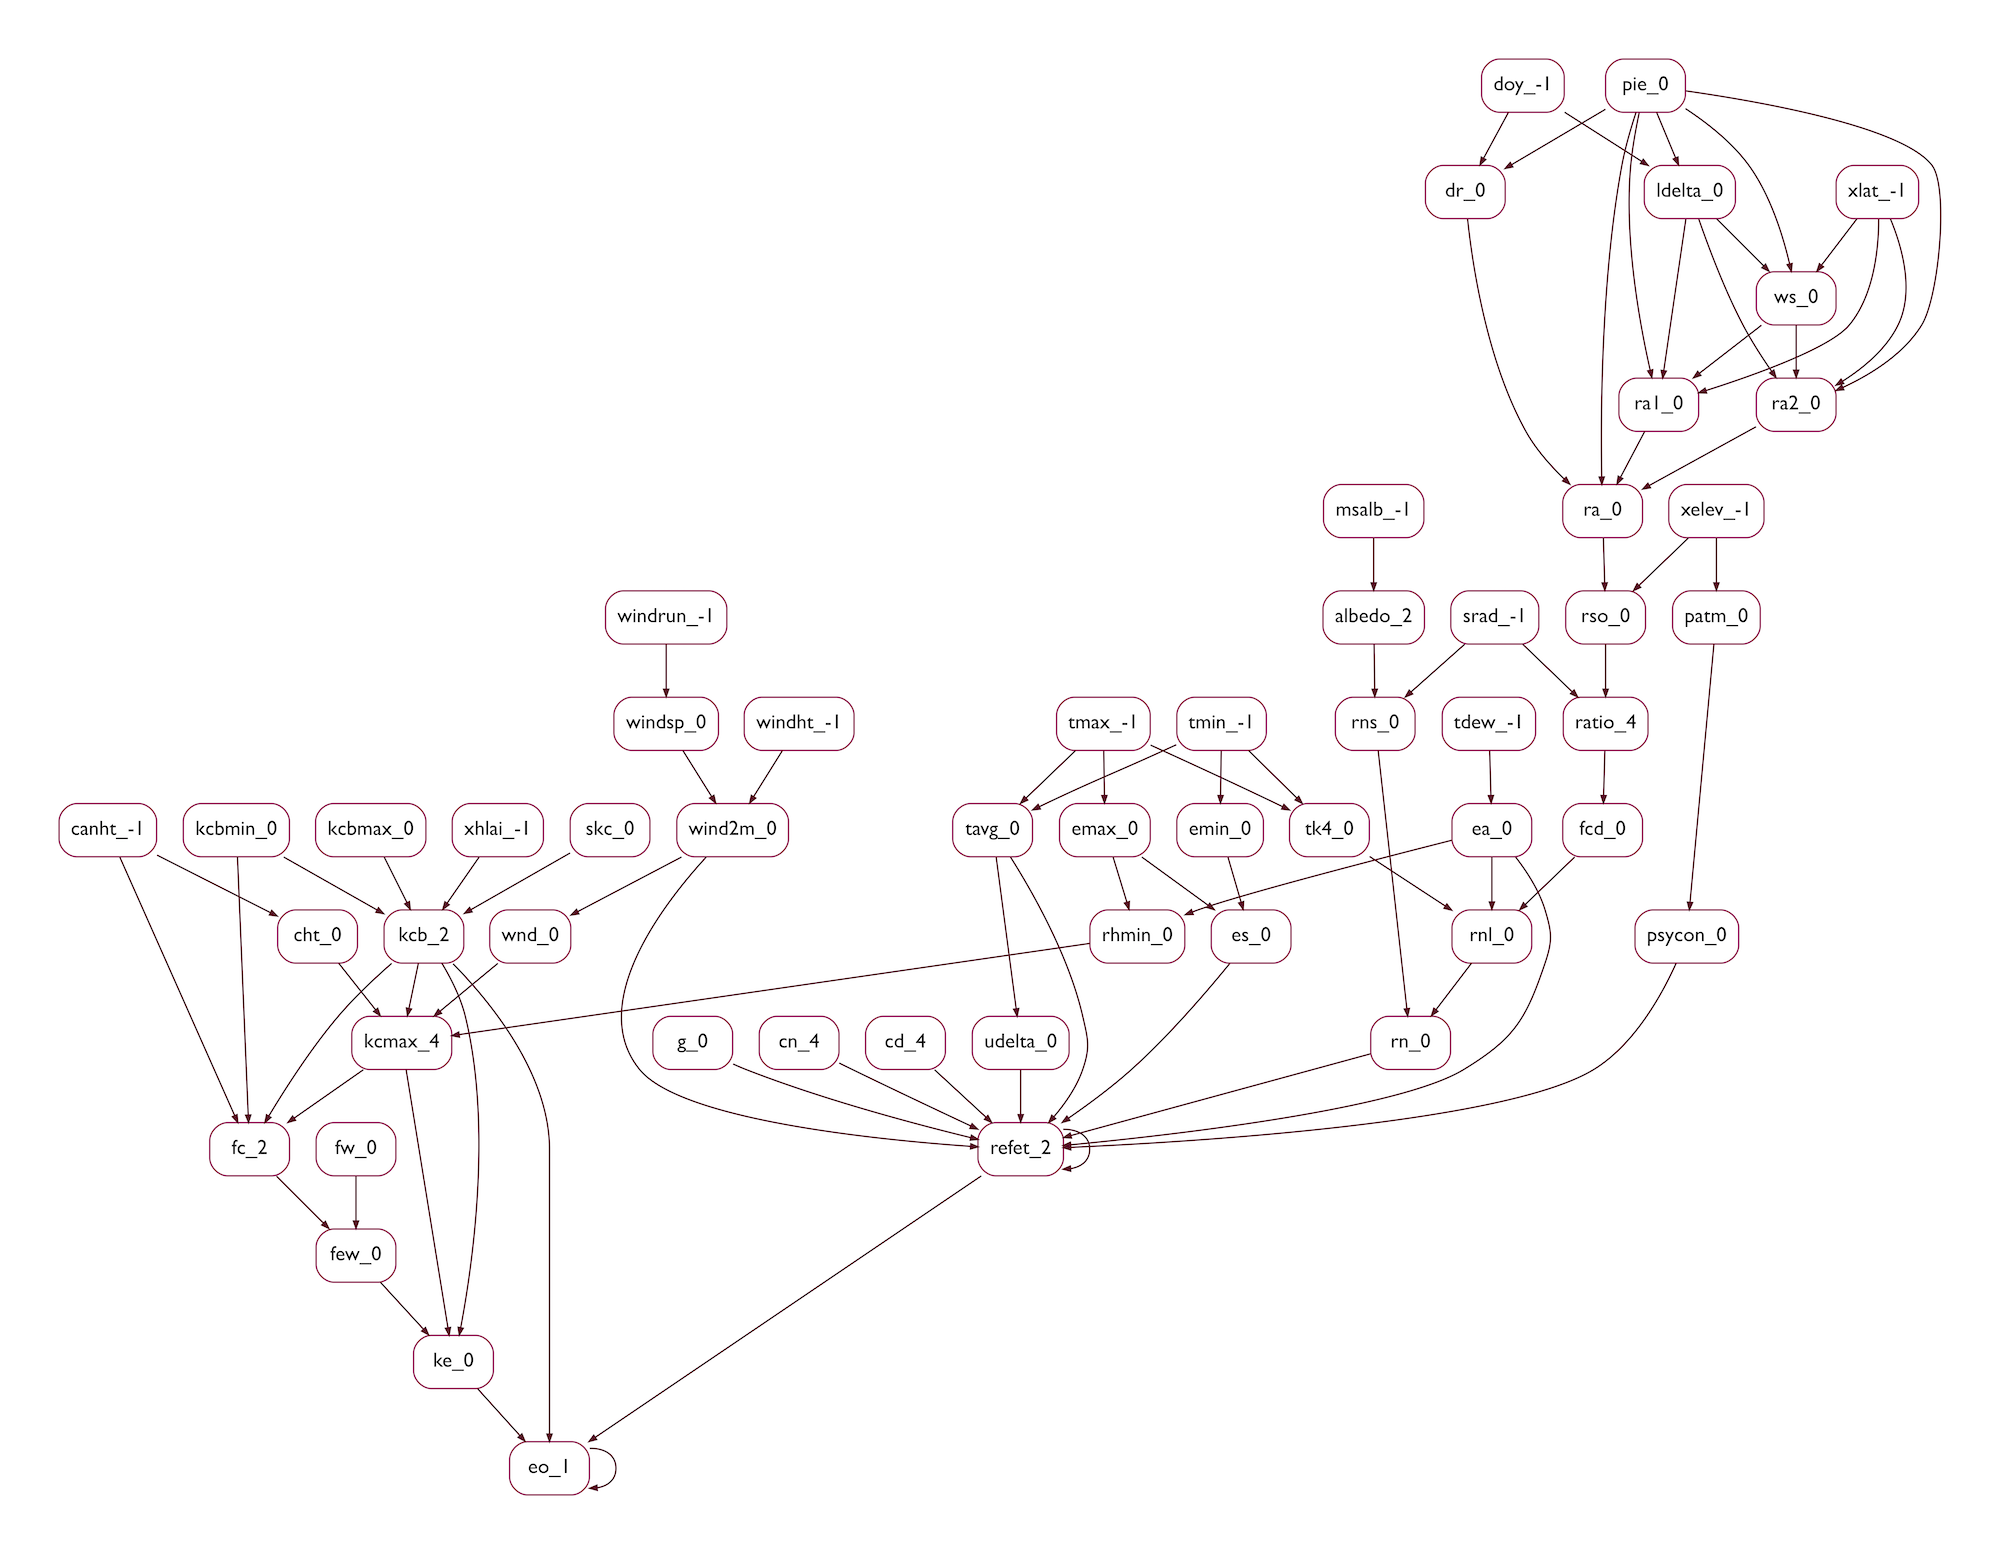
\includegraphics[width=0.75\textwidth]{PETASCE_GrFN_CAG_smaller}
    \label{fig:petasce_cag}
  }
  \caption[GrFN Causal Analysis Graph Examples]{Causal analysis graph views of the PETPT and PETASCE evapo-transpiration models.}
\end{figure}
\FloatBarrier

When treating the input variables as random variables we can induce a distribution over the values that they can take.
The distribution defined over the inputs will then induce a distribution onto the inner variable nodes and the output variable node of the GrFN CG.
For the GrFN CG to be a Dynamic Bayes Net (DBN) we need the probability distribution of the output variable to be a product of all of the input probability distributions \citep{pearl2009causality}.
During the computation of any inner variable in a GrFN CG we have a lambda function that denotes how the the inputs to the computation are to be combined to form the output.
All possible combinations are mathematical functions, that are able to be applied over the probability distribution of the inputs.
Therefore the resulting computed inner variable has a distribution that is the combination of the distributions over the inputs.
However, this distribution is not yet a probability distribution.
In order to create a probability distribution a normalization step is required so that the total probability mass sums to 1.
Once this step is complete we can see that we have satisfied the requirements for a DBN for the trivial case of a single computed node with a set of input nodes.
Since we are free to induce distributions on the input nodes of a GrFN, and all inner nodes and output nodes of a GrFN are defined in the same manner as the case explored above we can conclude that a GrFN CG is indeed a DBN.




\section{GrFN Computation Graph Evaluation Studies\label{sec:grfn_eval}}
% TODO: Finish writing this section
UMAF is a component of the AutoMATES pipeline, and as the AutoMATES team has been progressing more Fortran programs have been able to be parsed and translated into GrFNs.
This section details two evaluation studies that have been done upon the PA module and UMAF to determine the extent of Fortran constructs we are able to handle affectively, as well as how many scientific models found in DSSAT can be handled by UMAF.

\begin{table}
  \centering
  \label{tab:prog_idioms}
  \begin{tabular}{ |c|c| }
   \hline
   \textbf{Program Idiom} & \textbf{GrFN Representation Status} \\
   \hline
   Variable Declarations & Included \\
   Assignment Statement & Included \\
   Conditional Statement & Included \\
   Procedure Calls & Included \\
   Indexed Loops & Included \\
   Open-ended Loops & In Progress \\
   Case Statements & In Progress \\
   File I/O & In Progress \\
   Array Indexing & In Progress \\
   Derived Types & In Progress \\
   Multiple/Variable Outputs & Future \\
   Early Exit & Future \\
   Error Cases & Future \\
   \hline
  \end{tabular}
  \caption[GrFN Program Idiom Coverage]{Programming idiom coverage of the GrFN representation language. Note that many programming idioms may be absent from this table and others that are not normally included are present. This is due to the nature of GrFN as representing a subset of programs that are used to communicate scientific models and needing to represent programs in the form of a graphical model for inference.}
\end{table}

\begin{center}
  \begin{table}
    \centering
    \label{tab:pa_eval_table}
    \begin{tabular}{ |c|c|c|l| }
     \hline
     \textbf{Model Identifier} & \textbf{Parse Status} & \textbf{P,R,F1 Scores} & \textbf{Cause of Failure} \\
     \hline
     PETPT & \texttt{Success} & 1.0, 1.0, 1.0 & -- \\
     PETASCE & \texttt{Success} & 1.0, 1.0, 1.0 & -- \\
     \hline
     FLOOD\_EVAP & \texttt{Success} & 1.0, 1.0, 1.0 & -- \\
     SOLAR & \texttt{Success} & 1.0, 1.0, 1.0 & -- \\
     DECL & \texttt{Failure} & -- & User-defined functions \\
     INSOIL & \texttt{Failure} & -- & Unknown builtin functions (INDEX) \\
     PETPEN & \texttt{Failure} & -- & Variable declaration after assignment \\
     ROOTWU & \texttt{Failure} & -- & Iteration over non-constant range \\
     MULCH\_EVAP & \texttt{Failure} & -- & Use of derived types \\
     SNOWFALL & \texttt{Failure} & -- & Nested if-statements \\
     EFLOW\_C & \texttt{Failure} & -- & Early conditional exit \\
     ESUP & \texttt{Failure} & -- & Multiple/variable outputs \\
     \hline
    \end{tabular}
    \caption[Program Analysis Module Evaluation]{Evaluation results for the program analysis module. This evaluation tested the program analysis modules capability to parse and transfer correct GrFN representation wiring for 10 scientific models found in the DSSAT Fortran codebase.}
  \end{table}
\end{center}
